\chapter{Results and Discussion}
\label{ch:results}

\section{Results, Evaluation and Discussion}
This chapter presents the experiments in the order in which they were carried out, because each one explains the next: the production
model and its measured performance, a failure on genuine video, the diagnosis of that failure as an image-quality shortcut, an acceptance
gate, a retraining that fixed the video failure at a cost, and an experiment with modern generators. Every number comes from a saved result
file of the repository; the limits of each number are stated next to it.

\subsection{Experimental Setup and Dataset Partitioning}
\textbf{DeepFakeFace (DFF).} A sample of the dataset \citep{song2023dff} was used. The real images are IMDB-WIKI photographs
\citep{rothe2018imdbwiki}; for each real image one fake counterpart is generated by inpainting, face swapping (``insight'') or a text-to-image
model (``text2img''). Splits are identity- and pair-disjoint after duplicate removal (Table~\ref{tab:dffsplits}). The text-to-image fakes occur
only in the cross-generator test split, so that split measures behaviour on an \emph{unseen generator}.

\begin{table}[ht]
\centering
\caption{DeepFakeFace splits used for the production model (face crops).}
\label{tab:dffsplits}
\small
\begin{adjustbox}{max width=\linewidth,center}
\begin{tabular}{|l|p{3.4cm}|c|p{3.4cm}|}
\hline
\textbf{Split} & \textbf{Role} & \textbf{n (real / fake)} & \textbf{Fake generators} \\ \hline
train & fitting & 2{,}315 (1{,}170 / 1{,}145) & inpainting, insight \\ \hline
val & model selection & 471 (239 / 232) & inpainting, insight \\ \hline
test\_internal & unseen identities, seen generators & 575 (292 / 283) & inpainting, insight \\ \hline
test\_crossgen & unseen identities and unseen generator & 568 (281 / 287) & text2img \\ \hline
\end{tabular}
\end{adjustbox}
\end{table}

\textbf{Celeb-DF v2.} Videos \citep{li2020celebdf} were split by identity into training, validation and held-out test identities (nine test identities,
147 videos: 91 real and 56 fake); fakes whose source and target identities fall in different splits were dropped. Frames were sampled from
each video, cropped with the production detector and stored as JPEG. Test results are reported at frame level and at video level.

\textbf{Experiment E3 data.} Modern-generator data were added from FFHQ real faces \citep{karras2019stylegan}, SFHQ synthetic faces
\citep{sfhq2022} and the fake side of the DeepDetect-2025 collection (Table~\ref{tab:e3data}). The datasets were reviewed for provenance and
shortcuts before use (Appendix~\ref{app:datasets}); two candidate datasets were excluded.

\begin{table}[ht]
\centering
\caption[Composition of the experiment E3 manifest after face detection and near-duplicate removal]{Composition of the experiment E3 manifest after face detection and near-duplicate removal (crops).}
\label{tab:e3data}
\small
\begin{adjustbox}{max width=\linewidth,center}
\begin{tabular}{|p{3.3cm}|c|c|c|p{4.0cm}|}
\hline
\textbf{Source (label)} & \textbf{Train} & \textbf{Val.} & \textbf{modern\_test} & \textbf{Notes} \\ \hline
FFHQ (real) & 7{,}996 & 966 & 1{,}447 & file-disjoint, seed 42 \\ \hline
SFHQ (fake) & 3{,}000 & 473 & 677 & StyleGAN-generated \\ \hline
DeepDetect fake & 8{,}997 & 880 & 2{,}202 & modern generators; no per-image generator label \\ \hline
DeepFakeFace + Celeb-DF & as for Model 4 & as before & separate tests & original splits unchanged \\ \hline
\end{tabular}
\end{adjustbox}
\end{table}

\subsection{Performance Evaluation Methodology}
\textbf{Metrics.} With ``fake'' as the positive class the report uses accuracy, precision, recall, F1, the area under the ROC curve (ROC-AUC), the
false-positive rate (FPR: genuine faces called fake) and the false-negative rate (FNR: fakes called genuine), together with confusion matrices.
Intervals are Wilson 95\% intervals \citep{wilson1927} for rates and grouped-bootstrap intervals \citep{efron1993bootstrap} for the other metrics.

\textbf{Rules fixed in advance.} (i) The decision threshold is 0.5 and is never tuned. (ii) Model selection uses \emph{validation} data
only; test data are never used for selection or for thresholds. (iii) Results on held-out identities with seen generators (\emph{internal}) are always
reported separately from results on an unseen generator (\emph{cross-generator}). (iv) Celeb-DF results are \emph{within-dataset} evidence:
the held-out identities share the face-swap method and the footage type of the training videos, so they say nothing about other
manipulation methods. (v) Scores are raw sigmoid outputs, not probabilities.

\subsection{Results for the Production Model v2 (DeepFakeFace)}
The production model v2 was chosen among three training configurations by validation ROC-AUC alone (ImageNet initialisation, 9th epoch,
validation ROC-AUC 0.948); its test numbers were never consulted for selection. Table~\ref{tab:v2} shows its results.

\begin{table}[ht]
\centering
\caption[Production model v2 on DeepFakeFace (threshold 0.5; fake is positive; intervals are 95\%]{Production model v2 on DeepFakeFace (threshold 0.5; fake is positive; intervals are 95\% grouped bootstrap).}
\label{tab:v2}
\small
\begin{adjustbox}{max width=\linewidth,center}
\begin{tabular}{|l|c|c|c|c|c|c|}
\hline
\textbf{Split} & \textbf{Acc} & \textbf{Prec} & \textbf{Recall} & \textbf{F1} & \textbf{ROC-AUC} & \textbf{FPR / FNR} \\ \hline
Validation (selection) & 0.877 & 0.843 & 0.922 & 0.881 & 0.948 (0.928--0.965) & 0.167 / 0.078 \\ \hline
Internal test & 0.875 (0.848--0.902) & 0.860 & 0.890 & 0.875 & 0.941 (0.921--0.960) & 0.140 / 0.110 \\ \hline
Cross-generator test & 0.746 (0.716--0.778) & 0.818 & 0.641 & 0.719 & 0.849 (0.818--0.879) & 0.146 / 0.359 \\ \hline
\end{tabular}
\end{adjustbox}
\end{table}

\begin{figure}[ht]
\centering
\begin{subfigure}[t]{0.47\linewidth}\centering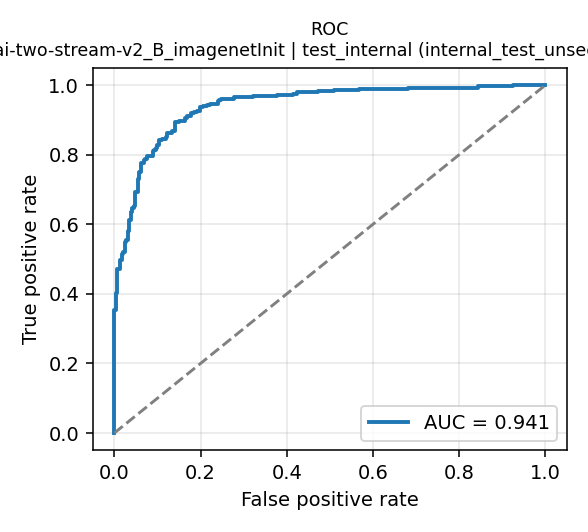
\includegraphics[width=\linewidth,height=0.9048\linewidth]{figures/v2_roc_test_internal.png}\caption{Internal test}\end{subfigure}\hfill
\begin{subfigure}[t]{0.47\linewidth}\centering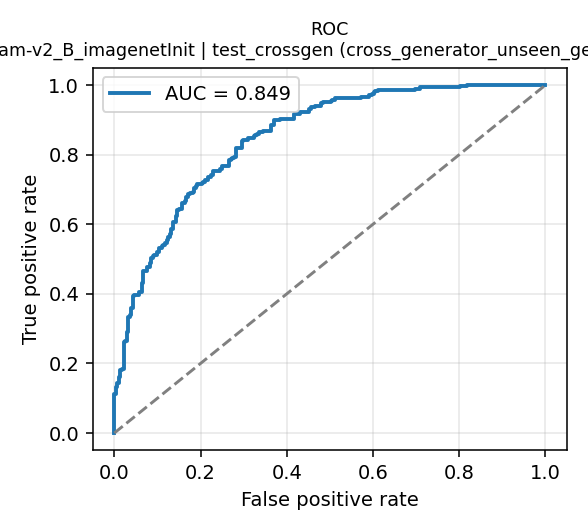
\includegraphics[width=\linewidth,height=0.9048\linewidth]{figures/v2_roc_test_crossgen.png}\caption{Cross-generator test}\end{subfigure}
\caption[ROC curves of v2 on the two held-out DeepFakeFace test splits (generated by the evaluation]{ROC curves of v2 on the two held-out DeepFakeFace test splits (generated by the evaluation script).}
\label{fig:v2roc}
\end{figure}

\begin{figure}[ht]
\centering
\begin{subfigure}[t]{0.47\linewidth}\centering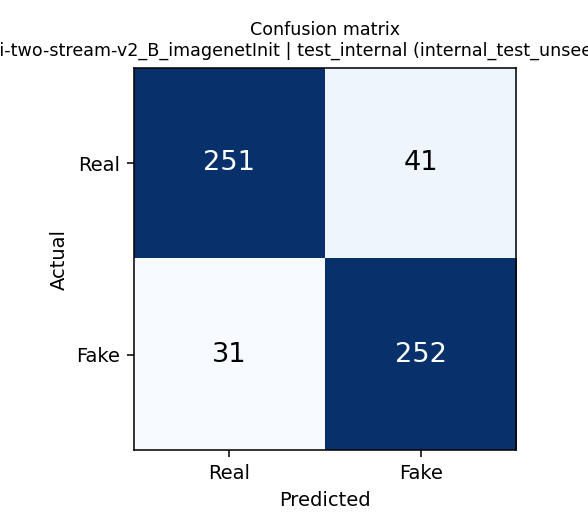
\includegraphics[width=\linewidth,height=0.9048\linewidth]{figures/v2_confusion_matrix_test_internal.png}\caption{Internal test}\end{subfigure}\hfill
\begin{subfigure}[t]{0.47\linewidth}\centering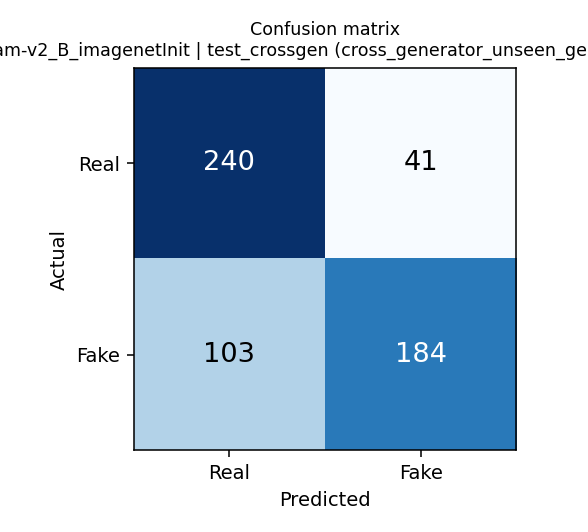
\includegraphics[width=\linewidth,height=0.9048\linewidth]{figures/v2_confusion_matrix_test_crossgen.png}\caption{Cross-generator test}\end{subfigure}
\caption[Confusion matrices of v2 at threshold 0.5]{Confusion matrices of v2 at threshold 0.5. On the unseen generator the model misses a much larger share of fakes (103 of 287).}
\label{fig:v2cm}
\end{figure}

On the internal split v2 detects inpainting fakes 91.5\% and face swaps 86.6\% of the time and accepts 85.9\% of real photographs. On the unseen
text-to-image generator the detection rate falls to 64.1\%. This gap between internal and cross-generator performance is the first
evidence that the measured accuracy depends on the generators seen during training, and \emph{the internal numbers must not be quoted as general accuracy}.
For comparison, the original prototype's checkpoint, evaluated on the same identity-disjoint data, performed at chance level; the very high accuracy
reported for the prototype could therefore not be reproduced under this protocol.

\subsection{A Failure on Genuine Video: the Four-Model Comparison}
When genuine video of a person was analysed with v2, the application sometimes reported FAKE with very high scores. To test this
systematically, four models were evaluated with identical code on the held-out Celeb-DF identities: Model~1 (production v2), Model~2 (DeepFakeFace only with
quality augmentation), Model~3 (DeepFakeFace plus Celeb-DF) and Model~4 (as Model 3 with quality augmentation). Table~\ref{tab:fourvideo} gives the video-level results.

\begin{table}[ht]
\centering
\caption[Video-level results on 147 held-out Celeb-DF videos (91 real, 56 fake), clean inputs, 95\%]{Video-level results on 147 held-out Celeb-DF videos (91 real, 56 fake), clean inputs, 95\% Wilson intervals.}
\label{tab:fourvideo}
\small
\begin{adjustbox}{max width=\linewidth,center}
\begin{tabular}{|l|c|c|c|}
\hline
\textbf{Model} & \textbf{Accuracy} & \textbf{FPR (real called fake)} & \textbf{FNR (fake called real)} \\ \hline
1 Production v2 & 0.483 (0.404--0.563) & 55/91 = 0.604 (0.502--0.699) & 21/56 = 0.375 (0.260--0.506) \\ \hline
2 DFF only + quality aug. & 0.578 (0.497--0.655) & 16/91 = 0.176 (0.111--0.267) & 46/56 = 0.821 (0.702--0.900) \\ \hline
3 DFF + Celeb-DF & 0.973 (0.932--0.989) & 4/91 = 0.044 (0.017--0.108) & 0/56 = 0.000 (0.000--0.064) \\ \hline
4 DFF + Celeb-DF + quality aug. & 0.980 (0.942--0.993) & 2/91 = 0.022 (0.006--0.077) & 1/56 = 0.018 (0.003--0.094) \\ \hline
\end{tabular}
\end{adjustbox}
\end{table}

The production model is at chance level on this video set (55 of 91 genuine videos called fake). Models trained on Celeb-DF frames reach
0.97--0.98 video accuracy, but this is \emph{within-dataset} evidence: the test identities share the face-swap method and the footage type of the training videos.
Adding Celeb-DF also had a cost on DeepFakeFace: Model 4's false-negative rate on the unseen generator rose from 0.359 (v2) to 0.634, and on the internal test from 0.110 to 0.201 (Table~\ref{tab:e3-frame}).

\subsection{Diagnosis: an Image-Quality Shortcut}
\label{sec:diag}
Experiment E1 measured whether image sharpness alone predicts the label (no model involved). In DeepFakeFace the fakes are softer than the real
photographs: the ROC-AUC of \emph{softness alone} as a classifier of FAKE is 0.712 (95\% CI 0.696--0.729) on the training split, 0.680 on the internal
test split and --- on the unseen generator --- \textbf{0.432}, i.e.\ the cue reverses. The share of fakes among crops rises from 26\% in the sharpest
bin to 85\% in the softest (Figure~\ref{fig:shortcut}). Celeb-DF frames are almost all very soft (about 94\% fall into the softest sharpness bin, against about 8\% of DeepFakeFace training crops), so a model trained on
DeepFakeFace alone has seen almost no soft real faces and learns ``soft face means fake'', which explains the false alarms on soft genuine video.
Stream-level analysis showed that the noise stream carries this dependence: the Spearman correlation between sharpness and the noise-stream score was $-0.36$
(real faces) and $-0.52$ (fake faces) for the production model on the DeepFakeFace internal test split, while the RGB stream's correlation was close to zero. On the
Celeb-DF validation faces the production model's noise stream alone called 98.7\% of the real faces fake (stage-0 diagnostics).

\begin{figure}[ht]
\centering
\begin{adjustbox}{max width=\linewidth,center}
\begin{tikzpicture}
\begin{axis}[width=0.92\linewidth,height=6.2cm,ybar,bar width=7pt,ymin=0,ymax=100,ylabel={Fake share of crops (\%)},
  symbolic x coords={{$<40$},{40--80},{80--160},{160--320},{$\ge320$}},xtick=data,xlabel={Sharpness bin (variance of Laplacian)},
  legend style={at={(0.5,1.02)},anchor=south,legend columns=3,font=\footnotesize},tick label style={font=\footnotesize},
  enlarge x limits=0.15,ymajorgrids]
\addplot[fill=navy!70] coordinates {({$<40$},85)({40--80},71)({80--160},56)({160--320},40)({$\ge320$},26)};
\addplot[fill=accent!70] coordinates {({$<40$},75)({40--80},71)({80--160},53)({160--320},39)({$\ge320$},30)};
\addplot[fill=orange!80] coordinates {({$<40$},22)({40--80},43)({80--160},44)({160--320},53)({$\ge320$},55)};
\legend{DFF train,DFF internal test,DFF cross-generator test}
\end{axis}
\end{tikzpicture}
\end{adjustbox}
\caption[Fake share per fixed sharpness bin in DeepFakeFace (values from the E1 diagnostic)]{Fake share per fixed sharpness bin in DeepFakeFace (values from the E1 diagnostic). In the training and internal splits softness predicts
``fake''; on the unseen generator the relation is reversed, which shows that sharpness is a dataset shortcut and not a manipulation cue.}
\label{fig:shortcut}
\end{figure}

\subsection{The Stage-0 Acceptance Gate}
Because overall accuracy hides this kind of failure, a per-quality-bin acceptance gate was designed and its thresholds were frozen in a
protocol document before any run. It checks that each stream separates the classes on its own (G1), that scores are not correlated with
sharpness within a class (G2), that error rates do not vary across quality bins (G3) and that the model separates the classes within bins (G4),
on validation data only, clean and with class-blind degradations. Synthetic controls validate the gate itself: a softness-only classifier
must fail it and a quality-independent scorer must not. All four models failed the gate (Table~\ref{tab:gate}); models 3 and 4 pass the
ungated screen (ROC-AUC $\ge0.90$ on both clean validation sets) yet fail the gate, which shows that the gate carries information that the aggregate metric does not.
The thresholds were chosen while reading E1 results that included test splits, so stage-0 cannot prove independence of its thresholds from the test data; this is stated as a limitation.

\begin{table}[ht]
\centering
\caption[Stage-0 gate results (validation data, clean and degraded sets; DFF = DeepFakeFace, CDF =]{Stage-0 gate results (validation data, clean and degraded sets; DFF = DeepFakeFace, CDF = Celeb-DF).}
\label{tab:gate}
\small
\begin{adjustbox}{max width=\linewidth,center}
\begin{tabular}{|l|c|p{6.0cm}|}
\hline
\textbf{Model} & \textbf{Passes ungated screen} & \textbf{Gate failures (set:check)} \\ \hline
1 Production v2 & no & 13 failures across DFF and CDF, clean and degraded \\ \hline
2 DFF only + quality aug. & no & 9 failures \\ \hline
3 DFF + Celeb-DF & yes & DFF-clean:G3; DFF-degraded:G1--G4; CDF-degraded:G2--G4 \\ \hline
4 DFF + Celeb-DF + quality aug. & yes & DFF-clean:G2; DFF-degraded:G1; CDF-degraded:G2 \\ \hline
\end{tabular}
\end{adjustbox}
\end{table}

\subsection{Experiment E3: Modern-Generator Training}
\label{sec:e3}
The protocol of E3 (data, leakage control, candidates, evaluation, promotion rule) was written \emph{before} training. Two candidates were
trained on the enlarged data with the Model-4 recipe: E3A with quality augmentation and E3B without. The choice between them used validation only
(E3A, validation selection score 0.980 against 0.939). Both were evaluated with Model 4 and v2 under the same protocol (Tables~\ref{tab:e3-frame}--\ref{tab:e3-mixed}).

\textbf{Reading the tables.} The ``Validation'' row is the \emph{combined} E3 validation split, which includes modern-generator and Celeb-DF crops
that Model 4 and v2 were never trained on; their low accuracy there reflects that mismatch and is not a regression. The E3 evaluation re-extracted the Celeb-DF crops, so
the Celeb-DF numbers differ slightly from the earlier four-model comparison (Model 4: video accuracy 0.980 in both; v2: 0.476 here against 0.483 there).

% generated by report/scripts/make_tables.py from docs/results/e3_modern/e3_selection.json
\begin{table}[ht]\centering\caption[Frame-level results, clean inputs, fixed threshold 0.5 (FPR: real called FAKE; FNR: fake called REAL; 95\% Wilson intervals)]{Frame-level results, clean inputs, fixed threshold 0.5 (FPR: real called FAKE; FNR: fake called REAL; 95\% Wilson intervals). Counts are real / fake crops.}\label{tab:e3-frame}\scriptsize\resizebox{\ifdim\width>\linewidth\linewidth\else\width\fi}{!}{\begin{tabular}{|l|l|c|c|c|c|c|}\hline
\textbf{Split} & \textbf{Model} & \textbf{n (R/F)} & \textbf{Acc} & \textbf{AUC} & \textbf{FPR} & \textbf{FNR} \\ \hline
Validation & E3A & 2045/2410 & 0.952 & 0.990 & 0.039 [0.03,0.05] & 0.056 [0.05,0.07] \\
 & E3B & 2045/2410 & 0.954 & 0.992 & 0.056 [0.05,0.07] & 0.037 [0.03,0.05] \\
 & Model 4 & 2045/2410 & 0.654 & 0.713 & 0.066 [0.06,0.08] & 0.583 [0.56,0.60] \\
 & v2 & 2045/2410 & 0.489 & 0.484 & 0.319 [0.30,0.34] & 0.675 [0.66,0.69] \\
\hline
DFF internal test & E3A & 292/283 & 0.833 & 0.916 & 0.106 [0.08,0.15] & 0.230 [0.18,0.28] \\
 & E3B & 292/283 & 0.861 & 0.939 & 0.130 [0.10,0.17] & 0.148 [0.11,0.19] \\
 & Model 4 & 292/283 & 0.835 & 0.921 & 0.130 [0.10,0.17] & 0.201 [0.16,0.25] \\
 & v2 & 292/283 & 0.875 & 0.941 & 0.140 [0.11,0.18] & 0.110 [0.08,0.15] \\
\hline
DFF cross-generator test & E3A & 281/287 & 0.643 & 0.793 & 0.085 [0.06,0.12] & 0.624 [0.57,0.68] \\
 & E3B & 281/287 & 0.729 & 0.850 & 0.089 [0.06,0.13] & 0.449 [0.39,0.51] \\
 & Model 4 & 281/287 & 0.627 & 0.795 & 0.107 [0.08,0.15] & 0.634 [0.58,0.69] \\
 & v2 & 281/287 & 0.746 & 0.849 & 0.146 [0.11,0.19] & 0.359 [0.31,0.42] \\
\hline
Celeb-DF test (frames) & E3A & 1453/895 & 0.954 & 0.989 & 0.046 [0.04,0.06] & 0.045 [0.03,0.06] \\
 & E3B & 1453/895 & 0.957 & 0.991 & 0.050 [0.04,0.06] & 0.032 [0.02,0.05] \\
 & Model 4 & 1453/895 & 0.953 & 0.988 & 0.038 [0.03,0.05] & 0.061 [0.05,0.08] \\
 & v2 & 1453/895 & 0.471 & 0.479 & 0.593 [0.57,0.62] & 0.425 [0.39,0.46] \\
\hline
modern\_test & E3A & 1447/2879 & 0.983 & 0.998 & 0.014 [0.01,0.02] & 0.019 [0.01,0.02] \\
 & E3B & 1447/2879 & 0.981 & 0.998 & 0.037 [0.03,0.05] & 0.011 [0.01,0.02] \\
 & Model 4 & 1447/2879 & 0.328 & 0.414 & 0.082 [0.07,0.10] & 0.969 [0.96,0.97] \\
 & v2 & 1447/2879 & 0.326 & 0.398 & 0.090 [0.08,0.11] & 0.968 [0.96,0.97] \\
\hline
\end{tabular}}\end{table}

\begin{table}[ht]\centering\caption[Video-level results on the Celeb-DF held-out identities (91 real and 56 fake videos), clean]{Video-level results on the Celeb-DF held-out identities (91 real and 56 fake videos), clean inputs.}\label{tab:e3-video}\small\resizebox{\ifdim\width>\linewidth\linewidth\else\width\fi}{!}{\begin{tabular}{|l|c|c|c|c|}\hline
\textbf{Model} & \textbf{Accuracy} & \textbf{ROC-AUC} & \textbf{FPR [95\% CI]} & \textbf{FNR [95\% CI]} \\ \hline
E3A & 0.980 & 1.000 & 0.022 [0.01,0.08] & 0.018 [0.00,0.09] \\ \hline
E3B & 0.980 & 0.999 & 0.022 [0.01,0.08] & 0.018 [0.00,0.09] \\ \hline
Model 4 & 0.980 & 0.998 & 0.011 [0.00,0.06] & 0.036 [0.01,0.12] \\ \hline
v2 & 0.476 & 0.479 & 0.604 [0.50,0.70] & 0.393 [0.28,0.52] \\ \hline
\end{tabular}}\end{table}

\begin{table}[ht]\centering\caption[Share of crops called FAKE per source, clean inputs (for real sources this is the]{Share of crops called FAKE per source, clean inputs (for real sources this is the false-positive rate; for fake sources it is the detection rate).}\label{tab:e3-pergen}\scriptsize\resizebox{\ifdim\width>\linewidth\linewidth\else\width\fi}{!}{\begin{tabular}{|l|l|c|c|c|c|c|}\hline
\textbf{Split} & \textbf{Source} & \textbf{n} & \textbf{E3A} & \textbf{E3B} & \textbf{Model 4} & \textbf{v2} \\ \hline
modern\_test & deepdetect\_fake & 2202 & 0.996 [0.99,1.00] & 0.997 [0.99,1.00] & 0.029 [0.02,0.04] & 0.028 [0.02,0.04] \\
 & real\_ffhq & 1447 & 0.014 [0.01,0.02] & 0.037 [0.03,0.05] & 0.082 [0.07,0.10] & 0.090 [0.08,0.11] \\
 & sfhq & 677 & 0.931 [0.91,0.95] & 0.963 [0.95,0.97] & 0.038 [0.03,0.06] & 0.044 [0.03,0.06] \\
\hline
test\_internal & inpainting & 141 & 0.780 [0.70,0.84] & 0.837 [0.77,0.89] & 0.787 [0.71,0.85] & 0.915 [0.86,0.95] \\
 & insight & 142 & 0.761 [0.68,0.82] & 0.866 [0.80,0.91] & 0.810 [0.74,0.87] & 0.866 [0.80,0.91] \\
 & real & 292 & 0.106 [0.08,0.15] & 0.130 [0.10,0.17] & 0.130 [0.10,0.17] & 0.140 [0.11,0.18] \\
\hline
test\_crossgen & real & 281 & 0.085 [0.06,0.12] & 0.089 [0.06,0.13] & 0.107 [0.08,0.15] & 0.146 [0.11,0.19] \\
 & text2img & 287 & 0.376 [0.32,0.43] & 0.551 [0.49,0.61] & 0.366 [0.31,0.42] & 0.641 [0.58,0.69] \\
\hline
cdf\_test & celebdf\_synthesis & 895 & 0.955 [0.94,0.97] & 0.968 [0.95,0.98] & 0.939 [0.92,0.95] & 0.575 [0.54,0.61] \\
 & real & 1453 & 0.046 [0.04,0.06] & 0.050 [0.04,0.06] & 0.038 [0.03,0.05] & 0.593 [0.57,0.62] \\
\hline
\end{tabular}}\end{table}

\begin{table}[ht]\centering\caption[Robustness to a class-blind \emph{mixed} degradation (blur, down-up resampling, JPEG, noise]{Robustness to a class-blind \emph{mixed} degradation (blur, down-up resampling, JPEG, noise, low light) applied identically to every crop.}\label{tab:e3-mixed}\small\resizebox{\ifdim\width>\linewidth\linewidth\else\width\fi}{!}{\begin{tabular}{|l|c|c|c|c|c|}\hline
\textbf{Model} & \textbf{modern\_test Acc} & \textbf{FPR} & \textbf{FNR} & \textbf{Celeb-DF video Acc} & \textbf{video FPR} \\ \hline
E3A & 0.945 & 0.080 & 0.043 & 0.973 & 0.033 \\ \hline
E3B & 0.767 & 0.241 & 0.229 & 0.973 & 0.044 \\ \hline
Model 4 & 0.343 & 0.142 & 0.915 & 0.973 & 0.011 \\ \hline
v2 & 0.414 & 0.397 & 0.680 & 0.388 & 0.725 \\ \hline
\end{tabular}}\end{table}

\begin{table}[ht]\centering\caption{The frozen promotion rule applied to E3A (rule written before training).}\label{tab:promo-e3a}\small\begin{tabular}{|c|p{5.2cm}|p{4.2cm}|c|}\hline
\textbf{\#} & \textbf{Criterion} & \textbf{Value} & \textbf{Result} \\ \hline
1 & Celeb-DF video FPR $\le$ Model 4's + 0.03 and accuracy $\ge0.95$ & FPR 0.022 vs 0.011; acc 0.980 & \textbf{PASS} \\ \hline
2 & DFF test\_internal: FNR $\le$ v2's + 0.05 and FPR $\le0.20$ & FNR 0.230 (limit 0.160); FPR 0.106 & \textbf{FAIL} \\ \hline
2 & DFF test\_crossgen: FNR $\le$ v2's + 0.05 and FPR $\le0.20$ & FNR 0.624 (limit 0.409); FPR 0.085 & \textbf{FAIL} \\ \hline
3 & modern\_test balanced accuracy $\ge$ Model 4's + 0.10, interval above 0 & 0.984 vs 0.475 (diff +0.509, lower bound +0.500) & \textbf{PASS} \\ \hline
\end{tabular}\end{table}


\Needspace{6\baselineskip}\textbf{Interpretation.}
\begin{itemize}
\item On \texttt{modern\_test} E3A and E3B detect almost all held-out modern fakes (about 98\% accuracy, FPR 0.014 and 0.037) whereas Model 4 and v2 detect
only a few percent of them. The improvement is large and the intervals do not overlap.
\item \textbf{This is not generator-disjoint evidence.} The fakes in \texttt{modern\_test} come from the same generator families as the training fakes
(DeepDetect carries no per-image generator labels), and its real faces are all FFHQ, so a ``FFHQ-versus-generated'' style shortcut cannot be excluded.
The only unseen-generator test is the DeepFakeFace cross-generator split, where E3A is not better than Model 4 (FNR 0.624 versus 0.634) and clearly worse than v2 (0.359).
\item Celeb-DF video accuracy is unchanged at 0.980; the noise-robustness of E3A under the mixed degradation is good on \texttt{modern\_test}, whereas E3B degrades strongly.
\item By the frozen promotion rule (Table~\ref{tab:promo-e3a}) E3A fails criterion 2 (DeepFakeFace detection must not be more than 0.05 worse than v2). The same criterion fails for Model 4. \textbf{E3A was therefore not promoted.}
\end{itemize}

\subsection{Experiment E4: Source-Balanced Variant}
\label{sec:e4}
Experiment E4 repeats every DeepFakeFace \emph{training} row four times (validation and test unchanged) in the E3A recipe (ImageNet initialisation, quality augmentation 0.5, AdamW $10^{-4}$, batch 32, at most 12 epochs, seed 42),
to test whether source imbalance (DeepFakeFace is about 5\% of the training fakes) causes the loss of DeepFakeFace detection. The protocol and the promotion rule were registered before training. The run took 134.5 minutes on the Kaggle T4: all 12 epochs ran and the best epoch (by validation selection score) was epoch 12 (0.9797; validation accuracy 0.954, ROC-AUC 0.990), so training had not plateaued. Table~\ref{tab:e4-key} gives the held-out test results
(same splits and evaluation code as E3) and Table~\ref{tab:promo-e4a} applies the promotion rule.

% generated by report/scripts/make_e4_tables.py from report/data/e4_selection.json
\begin{table}[ht]\centering\caption[Experiment E4 against Model 4 and v2: held-out results]{Experiment E4 against Model 4 and v2: held-out results, clean inputs, fixed threshold 0.5 (accuracy/ROC-AUC/FPR/FNR).}\label{tab:e4-key}\footnotesize
\begin{adjustbox}{max width=\linewidth,center}\begin{tabular}{|l|c|c|c|}\hline \textbf{Test set} & \textbf{E4} & \textbf{Model 4} & \textbf{v2} \\ \hline
DFF internal test (frames) & 0.831/0.908/0.130/0.208 & 0.835/0.921/0.130/0.201 & 0.875/0.941/0.140/0.110 \\ \hline
DFF cross-generator test (frames) & 0.688/0.799/0.110/0.509 & 0.627/0.795/0.107/0.634 & 0.746/0.849/0.146/0.359 \\ \hline
Celeb-DF test (frames) & 0.945/0.985/0.061/0.045 & 0.953/0.988/0.038/0.061 & 0.471/0.479/0.593/0.425 \\ \hline
Celeb-DF test (\textbf{video}) & 0.980/0.999/0.022/0.018 & 0.980/0.998/0.011/0.036 & 0.476/0.479/0.604/0.393 \\ \hline
modern\_test (frames) & 0.983/0.998/0.023/0.014 & 0.328/0.414/0.082/0.969 & 0.326/0.398/0.090/0.968 \\ \hline
\end{tabular}\end{adjustbox}\end{table}

\begin{table}[ht]\centering\caption{The frozen promotion rule applied to E4 (rule written before training).}\label{tab:promo-e4a}\small\begin{adjustbox}{max width=\linewidth,center}\begin{tabular}{|c|p{5.2cm}|p{4.2cm}|c|}\hline
\textbf{\#} & \textbf{Criterion} & \textbf{Value} & \textbf{Result} \\ \hline
1 & Celeb-DF video FPR $\le$ Model 4's + 0.03 and accuracy $\ge0.95$ & FPR 0.022 vs 0.011; acc 0.980 & \textbf{PASS} \\ \hline
2 & DFF test\_internal: FNR $\le$ v2's + 0.05 and FPR $\le0.20$ & FNR 0.208 (limit 0.160); FPR 0.130 & \textbf{FAIL} \\ \hline
2 & DFF test\_crossgen: FNR $\le$ v2's + 0.05 and FPR $\le0.20$ & FNR 0.509 (limit 0.409); FPR 0.110 & \textbf{FAIL} \\ \hline
3 & modern\_test balanced accuracy $\ge$ Model 4's + 0.10, interval above 0 & 0.982 vs 0.475 (diff +0.507, lower bound +0.498) & \textbf{PASS} \\ \hline
\end{tabular}\end{adjustbox}\end{table}


\textbf{Interpretation.} (i) Repeating the DeepFakeFace rows recovered \emph{part} of the unseen-generator detection (FNR 0.509 against 0.634 for Model 4 and 0.624 for E3A) and slightly improved the internal test (FNR 0.208 against 0.230 for E3A), but it did not reach v2
(0.110 and 0.359). (ii) Celeb-DF video accuracy (0.980) and \texttt{modern\_test} accuracy (0.983) are the same as for E3A. (iii) By the frozen rule E4 passes criteria 1 and 3 but \textbf{fails criterion 2} (internal FNR 0.208 against a limit of 0.160;
cross-generator FNR 0.509 against 0.409), so \textbf{E4 did not pass the project's production-promotion rule}. The earlier caveats still apply: \texttt{modern\_test} is not generator-disjoint, Celeb-DF is within-dataset evidence, and E4 is a single run (one seed).

\textbf{Final model configuration.} E4 has the same architecture as every other model (two EfficientNet-B0 streams, 11{,}972{,}954 parameters; Chapter~\ref{ch:design}) and the same preprocessing, threshold and scoring; only its training data and recipe differ. It is the latest trained model and combines the strongest held-out results on Celeb-DF video (0.980) and \texttt{modern\_test} (0.983) with a smaller DeepFakeFace loss than Model 4 on the unseen generator, but it does not beat every model on every split: v2 remains best on DeepFakeFace (0.875 and 0.746). By decision of the project owner, \textbf{E4 is the default model of the local examiner demonstration}; Model 4 is an alternative, selectable in the dashboard, and v2 is the rollback model. Because E4 did not pass the promotion rule it has \emph{not} replaced v2 on the public deployment: the free-tier host (512\,MB, no disk) cannot hold the checkpoint or two models, so the live API still serves v2. Results and PDF reports record the model name, role and checkpoint hash.


\subsection{Qualitative Analysis of Grad-CAM Output}
The heat-maps in Figures~\ref{fig:viewer} and \ref{fig:frames} show typical behaviour for a genuine public-domain portrait: the activation concentrates on
the forehead and hairline area and is weak over the central face. This kind of localisation is an \emph{explanation of what the RGB stream used}; it does not show where a
manipulation happened and it says nothing about the noise stream. Because both the quality shortcut and the generator-specific cues are present in the training
data, a plausible-looking heat-map cannot by itself be taken as evidence that the model uses manipulation artefacts.

\subsection{Verification of the Deployed System}
The end-to-end suite of nine browser tests passed against the local server, against a separately hosted frontend origin (which also verified cross-origin
access, PDF download and deletion), and against the public deployment (Vercel frontend and Render API). On the public deployment, image analysis and video analysis with the public test media
completed, the verdict, scores, face tracks, timeline selection, PDF download and deletion worked, direct navigation and a page refresh kept the same page, and no console errors
occurred. With Grad-CAM switched off on the free tier the viewers showed the explicit ``not available'' state. The public API returned the v2 checkpoint
(hash prefix 3b947755) and an empty history list, as configured. The public deployment is a restricted demonstration; Section~\ref{sec:deploy-impl} lists its limits.

\textbf{Informal checks with private media.} After the models were frozen, a small set of private demonstration files (genuine and AI-generated photographs and videos) was scored locally as a sanity check.
They were never used for training, threshold choice or model selection, were never uploaded, and are \emph{not} reported here for privacy; the set is too small and uncontrolled to count as an evaluation, and one file was a near-duplicate
of a training crop.

\subsection{Limitations and Threats to Validity}
\label{sec:limits}
\begin{itemize}
\item \textbf{Face-level, image-trained model.} The model analyses cropped faces; video is handled by aggregating frame scores with an unvalidated rule.
No labelled modern AI-video data were available, so \textbf{nothing is claimed about AI-generated video.}
\item \textbf{Generator and source overlap.} Internal splits share generators with the training data; \texttt{modern\_test} shares generator families and has a single real source.
The unseen-generator evidence rests on one dataset split (text-to-image faces from DeepFakeFace).
\item \textbf{Shortcuts.} Sharpness is a measured shortcut; resolution, file format and the source of the real class can also act as shortcuts, and
only some were controlled. Quality augmentation reduced but did not remove the dependence.
\item \textbf{Celeb-DF.} Results are within-dataset and use one manipulation method.
\item \textbf{Calibration.} Scores are raw sigmoid outputs and must not be read as probabilities; the INCONCLUSIVE band is a reporting rule, not a calibration.
\item \textbf{Explanations.} Grad-CAM indicates influential regions of the RGB stream; it does not prove manipulation.
\item \textbf{Real photographs.} Real images come from IMDB-WIKI, FFHQ and YouTube footage; modern phone photographs, webcams and heavy compression are under-represented, and demographic bias was not characterised.
\item \textbf{Model metadata.} The checkpoint metadata of Model 4 and E4 lists DeepFakeFace as training data although Celeb-DF was also used; checkpoints are kept unchanged.
\item \textbf{Deployment.} The public instance runs a different (older) checkpoint without heat-maps, has no persistent storage, no authentication and no rate limiting, and a 512\,MB limit makes long videos unreliable. It is not production-ready.
\item \textbf{Threshold of the gate.} The stage-0 thresholds were set with knowledge of earlier test-split diagnostics (disclosed in its protocol).
\end{itemize}

\subsection{Summary of Results}
\begin{enumerate}
\item The two-stream detector works well on the data it was trained on (v2: accuracy 0.875 internal), degrades on an unseen generator (0.746) and failed on genuine video.
\item The failure was traced to an image-quality shortcut; adding Celeb-DF video and quality augmentation (Model 4) reached 0.980 video accuracy on held-out Celeb-DF identities, at the price of weaker DeepFakeFace detection.
\item Adding modern-generator data (E3) lets the model detect held-out fakes of those generators, but without a generator-disjoint test this is not evidence of general detection, and it did not meet the pre-registered promotion rule; the source-balanced variant E4 recovered only part of the DeepFakeFace detection and did not meet it either.
\item No result supports a claim of 95\% (or any fixed) accuracy for modern AI-generated images or videos in general.
\end{enumerate}
